\chapter{Die Problemstellung - Segmentierung als Optimierungsproblem}
\label{sec:prob}
	
	\section{Grundlegendes über Bildverarbeitung}
	\label{sec:bild-basics}
	
	Bevor das Thema dieser Arbeit erläutert werden kann, muss zunächst der Rahmen gesteckt werden. Dies bedeutet unter anderem, dass der Begriff Bildverarbeitung definiert werden muss - aber was ist das denn nun konkret? Tatsächlich gibt es hier keine einheitliche Definition - das liegt unter anderem daran, dass die Grenzen zwischen Bildverarbeitung und maschinellem Sehen nicht klar abgesteckt werden können. Eine mögliche Definition wird von Rafael C. Gonzalez und Richard E. Woods in ihrem Buch \textit{Digital Image Processing} \cite[S. 1--3]{gonzalez-woods} beschrieben. Hierzu nehmen sie zunächst eine Unterscheidung von rechnergestützten Prozessen wie folgt vor: 
	\begin{description}
		\item[Low-Level] Darunter fallen einfache Operationen direkt am Bild, wie zum Beispiel Rauschreduktion oder die Erhöhung des Kontrastes. Input sowie Output sind jeweils durch ein Bild gegeben.
		\item[Mid-Level] Diese Kategorie von Prozessen zeichnet sich dadurch aus, dass aus einem Bild bestimmte Eigenschaften/Bereiche extrahiert werden, um daraus eine Information zu gewinnen. Exemplarisch hierfür kann die Segmentierung angeführt werden, die in dieser Arbeit mit Hilfe des in Abschnitt \ref{sec:de} vorgestellten Algorithmus realisiert werden soll. Während der Input aus einem ganzen Bild besteht, beläuft sich der Output lediglich auf einen Teil davon beziehungsweise ein bestimmtes Attribut des Bildes.
		\item[High-Level] Hier werden die aus den Mid-Level Prozessen erhaltenen Informationen verwendet, um bestimmte Aktionen auszulösen (z.B. im Bezug auf maschinelles Sehen)
	\end{description}
	
	Auf dieser Grundlage definieren Gonzales und Woods \cite[S. 1--3]{gonzalez-woods} den Terminus der Bildverarbeitung als Menge aller Low- und Mid-Level Prozesse. \\
	
	Einen in der heutigen Zeit zentralen Anwendungsfall für die Bildverarbeitung stellt \gls{ocr} dar. Wie der Name bereits vermuten lässt, ist das Ziel der \gls{ocr}, Zeichen oder Formen aus digitalen Bildern zu extrahieren und weiterzuverarbeiten. Schon in den frühen 1950ern - so bei \cite{cher-et-al-ocr} - haben Forscher nach Möglichkeiten gesucht, auf Papier befindlichen Text rechnergestützt einzulesen, um dem Menschen die mühselige Arbeit des manuellen Abtippens von Dokumenten abzunehmen. Abbildung \ref{fig:ocr-system} illustriert hierbei die typischen Vorgänge in einem \gls{ocr}-System. 
	
	\begin{figure}[H]
		\centering
		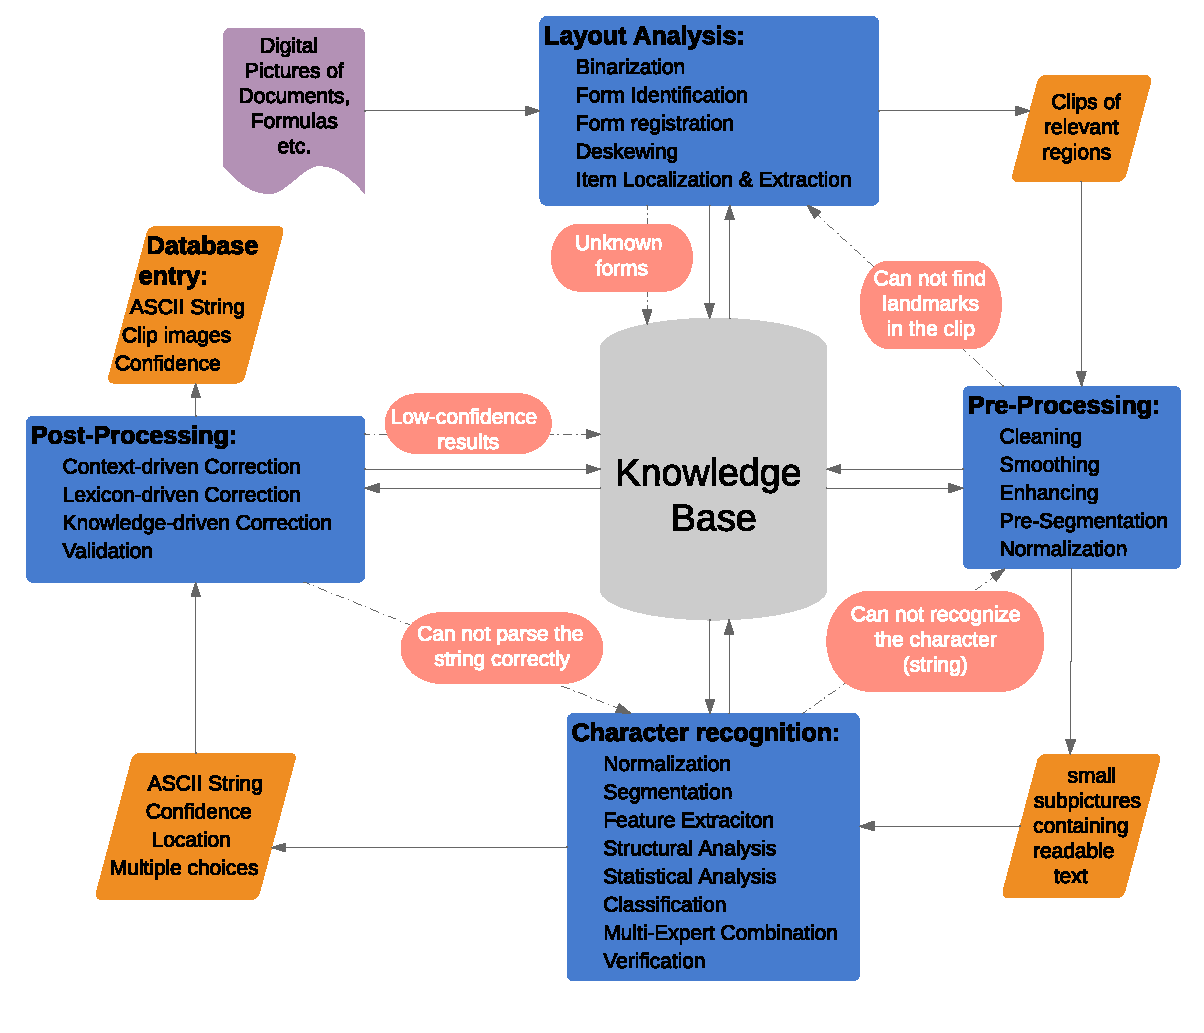
\includegraphics[width=0.7\linewidth]{Ablauf-OCR_Cheriet-et-al}
		\caption[typisches \gls{ocr}-Ablaufschema]{Schematische Darstellung des Ablaufs in einem intelligenten \gls{ocr}-System (aus \cite{cher-et-al-ocr})}
		\label{fig:ocr-system}
	\end{figure}

	Damit ein solches System zuverlässig Zeichen erkennen kann, muss es einerseits auf die Formen der Zeichen trainiert werden und andererseits als Input ein für die Anwendung angemessen segmentiertes Bild erhalten. Die Segmentierung ist eine Operation, die unterschiedliche Bereiche im Bild kennzeichnet, und hat nach \cite[S. 690 f]{gonzalez-woods}
	die folgenden Eigenschaften:
	\begin{itemize}
		\item Sei $R$ der Raum, den ein Bild einnimmt, bzw. das Bild selbst.
		\item Dann unterteilt die Segmentierung $R$ in $n$ Regionen $R_{i}$, sodass $\bigcup\limits_{i=1}^{n} R_{i} = R$, also dass die Vereinigung aller Teilregionen wieder das gesamte Bild ergibt
		\item Weiterhin ist $R_{i} \bigcap R_{j} = \emptyset $ für alle $i, j \in [1, ... , n]$ und $i \neq j$. \\
		D.h., die einzelnen Teilregionen sind disjunkt zueinander.
	\end{itemize}
		